\clearpage
\section{Durchführung}
\subsection{Versuchsaufbau}
Der Aufbau wird in der nachfolgenden Grafik illustriert.
\begin{figure}[h]
\begin{center}
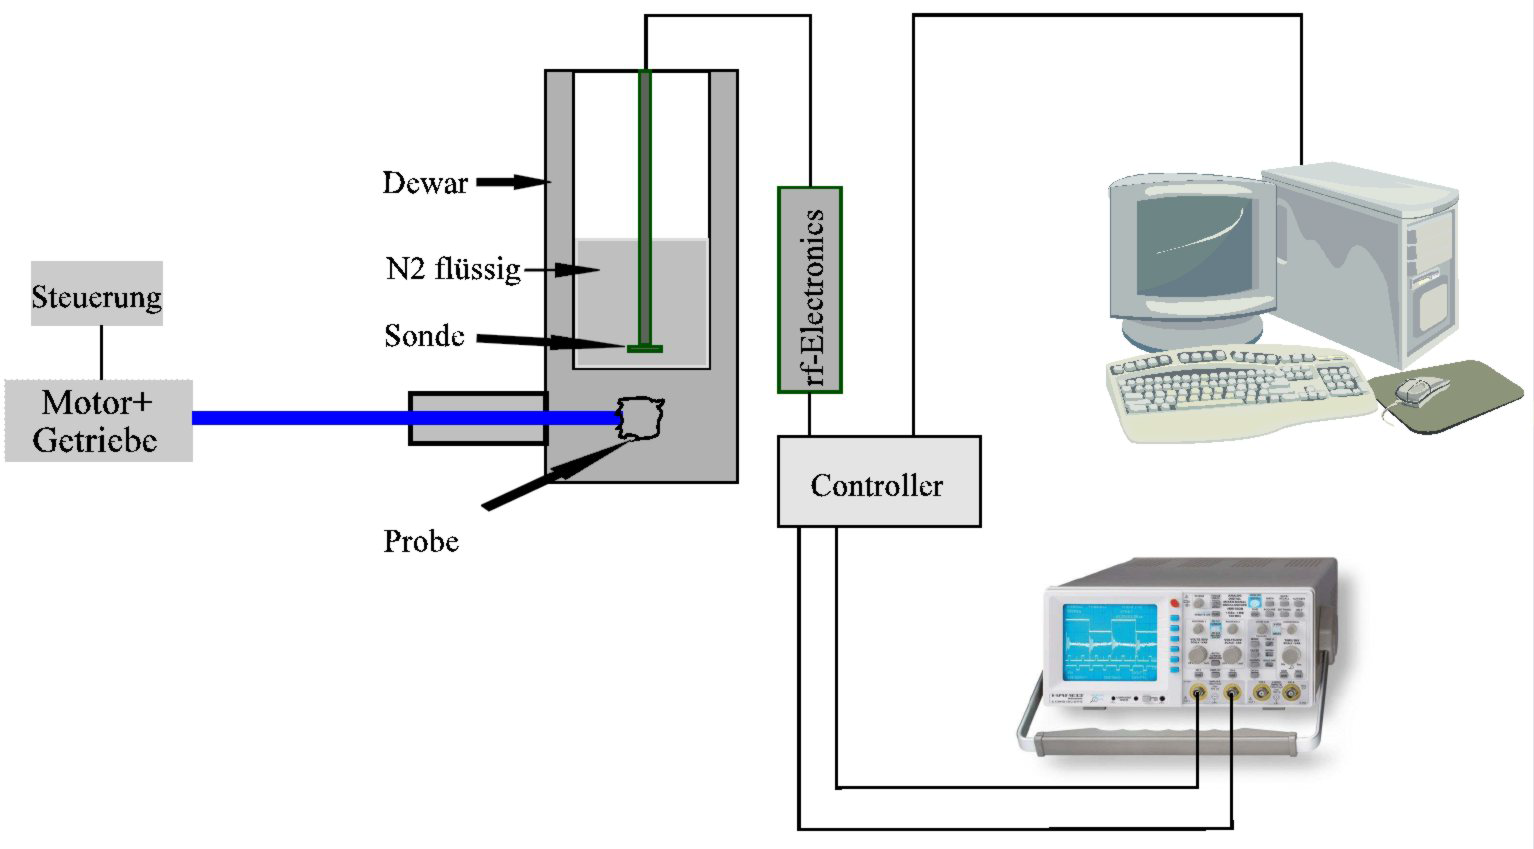
\includegraphics[scale=0.45]{aufbau}
\caption{Aufbau zum Versuch. Quelle: [ver]}
\label{fig:aufbau}
\end{center}
\end{figure}
\clearpage
\subsection{Erklärung zur Messanordnung}
Das Licht des HeNe-Lasers wird an einem Strahlteiler geteilt, wobei der abgelenkte Strahl auf einen Umlenkspiegel geleitet wird, welcher diesen direkt auf den Drehspiegel mit Motor leitet. Von dort aus wird der Strahl auf die Diode 2 eingestellt, welche so das Trigger-Signal angibt. Der Strahl, welcher den Strahlteiler ohne Ablenkung passiert wird durch eine Anordnung von zwei Linsen, deren Abstand genau der Summe ihrer Brennweiten entspricht, aufgeweitet. Mit der Blende kann die Beleuchtung der 'Gitter' kontrolliert werden. Auf die Blenden folgen die Gitter bzw. der Tank mit dem Isooktan. Durch die dritte Linse nach dem Gitter wird der Strahl auf die Diode fokussiert. Durch den Spiegel mit dem Motor kann das räumliche Interferenzmuster als eine zeitliche Intensitätsverteilung am Oszilloskop dargestellt werden.
\subsection{Messmethoden}
\subsubsection*{Aufgabe 1}
Für die Messung mit dem Sinusgitter wird der Laserstrahl ohne Aufweitung und ohne Kollimation direkt auf das Sinusgitter gerichtet. Auf einem Schirm hinter dem Gitter wird der Abstand vom nullten zu den ersten Maxima direkt vermessen.
\subsubsection*{Aufgabe 2}
Hier wird der oben beschriebene Aufbau verwendet. Es muss darauf geachtet werden, dass das Strahlenbündel parallel verläuft und senkrecht auf das Gitter trifft. Es werden hier nur die Gitter benutzt und nicht die Ultraschallzelle.
Damit Diode 1 nicht auch noch das Trigger-Signal erfasst werden die beiden Strahlen in der Höhe schoben. Die Dioden werden in der Höhe ihrem Strahl angepasst. Es genügt den Verstärker auf eine 10-fache Verstärkung zu betreiben.\\
Zunächst wird die Zeitachse am Oszilloskop mit einem Eichgitter, hier ein PHYWE -Gitter, geeicht werden. Nun werden für alle Beugungsordnungen die am Oszilloskop zeitlichen Abstände der Maxima vom Hauptmaxima bestimmt.
\subsubsection*{Aufgabe 3}
Für die Bestimmung der Aperturfunktion wird das Gitter mit der größten Anzahl an sichtbaren Beugungsordnungen benutzt.
\subsubsection*{Aufgabe 4}
Hierfür muss keine Messung vorgenommen werden.
\subsubsection*{Aufgabe 5}
Die Ultraschallzelle wird nun in den Aufbau integriert und an den Generator angeschlossen. Es wird zunächst bei $0V$ eine Frequenz bestimmt, bei der eine maximale erzielbare Anzahl an Maxima angezeigt wird und das Signal möglichst stabil ist. Diese Frequenz muss für alle Messungen in diesem Versuchsteil konstant bleiben.\\
Es werden für zehn verschiedene Spannungen Beugungsbilder an der Ultraschallzelle aufgenommen. Um eine Normierung vorzunehmen wird zusätzlich noch die Intensität des Strahls bei einer Spannung von $0V$ aufgenommen.
 